\documentclass[tikz,border=4pt]{standalone}
\usepackage[T1]{fontenc}
\usepackage[scaled=0.92]{helvet}
\usepackage{amsmath,amssymb}
\usepackage{tikz}
\usetikzlibrary{arrows.meta,positioning,shapes.geometric,calc}

\begin{document}
\sffamily
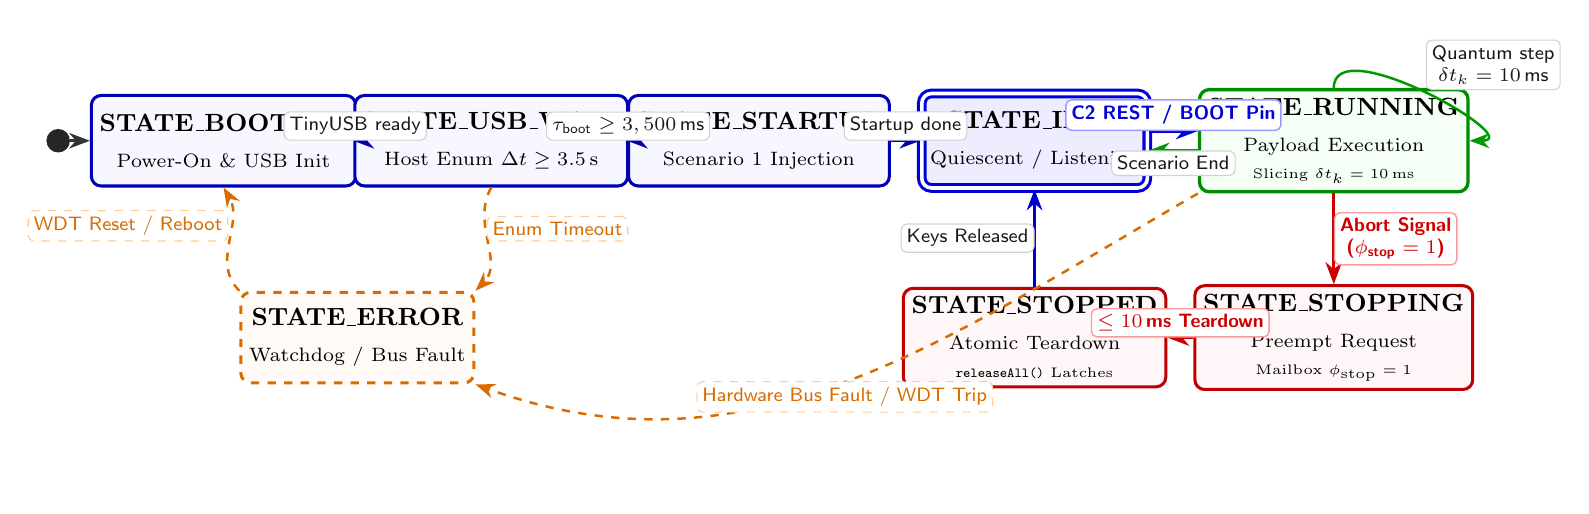
\begin{tikzpicture}[
    >=Stealth,
    font=\small,
    % Standard Operational State
    st_norm/.style={
        rectangle,
        rounded corners=3.5pt,
        draw=blue!70!black,
        line width=1.1pt,
        fill=blue!3!white,
        minimum width=2.45cm,
        minimum height=1.15cm,
        inner sep=3pt,
        align=center
    },
    % Idle State (Double Border Hub)
    st_idle/.style={
        rectangle,
        rounded corners=3.5pt,
        draw=blue!85!black,
        double,
        double distance=1.3pt,
        line width=1.1pt,
        fill=blue!7!white,
        minimum width=2.55cm,
        minimum height=1.2cm,
        inner sep=3pt,
        align=center
    },
    % Active Running State
    st_run/.style={
        rectangle,
        rounded corners=3.5pt,
        draw=green!55!black,
        line width=1.2pt,
        fill=green!4!white,
        minimum width=2.55cm,
        minimum height=1.15cm,
        inner sep=3pt,
        align=center
    },
    % Emergency Preempt / Stop States
    st_stop/.style={
        rectangle,
        rounded corners=3.5pt,
        draw=red!75!black,
        line width=1.1pt,
        fill=red!3!white,
        minimum width=2.45cm,
        minimum height=1.15cm,
        inner sep=3pt,
        align=center
    },
    % Error / Fault State
    st_err/.style={
        rectangle,
        rounded corners=3.5pt,
        draw=orange!85!black,
        line width=1.1pt,
        dashed,
        fill=orange!4!white,
        minimum width=2.45cm,
        minimum height=1.15cm,
        inner sep=3pt,
        align=center
    },
    % Edge Badges
    lbl/.style={
        font=\sffamily\scriptsize,
        fill=white,
        draw=gray!35,
        line width=0.4pt,
        rounded corners=2pt,
        inner sep=2pt,
        align=center,
        text=black!90
    },
    lbl_blue/.style={
        font=\sffamily\scriptsize\bfseries,
        fill=white,
        draw=blue!40,
        line width=0.5pt,
        rounded corners=2pt,
        inner sep=2pt,
        align=center,
        text=blue!85!black
    },
    lbl_red/.style={
        font=\sffamily\scriptsize\bfseries,
        fill=white,
        draw=red!40,
        line width=0.5pt,
        rounded corners=2pt,
        inner sep=2pt,
        align=center,
        text=red!80!black
    },
    lbl_amber/.style={
        font=\sffamily\scriptsize,
        fill=white,
        draw=orange!40,
        line width=0.4pt,
        rounded corners=2pt,
        inner sep=2pt,
        align=center,
        text=orange!85!black
    }
]

% Start Token
\node[circle, fill=black!85, inner sep=3pt] (start) at (-0.2, 0) {};

% Top Row: Main Execution Expressway
\node[st_norm] (boot)    at (1.9, 0) {\textbf{STATE\_BOOTING}\\[2pt]\scriptsize Power-On \& USB Init};
\node[st_norm] (usbwait) at (5.3, 0) {\textbf{STATE\_USB\_WAIT}\\[2pt]\scriptsize Host Enum $\Delta t \ge 3.5$\,s};
\node[st_norm] (startup) at (8.7, 0) {\textbf{STATE\_STARTUP}\\[2pt]\scriptsize Scenario 1 Injection};
\node[st_idle] (idle)    at (12.2, 0) {\textbf{STATE\_IDLE}\\[2pt]\scriptsize Quiescent / Listening};
\node[st_run]  (running) at (16.0, 0) {\textbf{STATE\_RUNNING}\\[2pt]\scriptsize Payload Execution\\[-1pt]\tiny Slicing $\delta t_k = 10$\,ms};

% Bottom Row: Fault Recovery (Left) & Preemption / Teardown (Right)
\node[st_err]  (error)    at (3.6, -2.5) {\textbf{STATE\_ERROR}\\[2pt]\scriptsize Watchdog / Bus Fault};
\node[st_stop] (stopped)  at (12.2, -2.5) {\textbf{STATE\_STOPPED}\\[2pt]\scriptsize Atomic Teardown\\[-1pt]\tiny \texttt{releaseAll()} Latches};
\node[st_stop] (stopping) at (16.0, -2.5) {\textbf{STATE\_STOPPING}\\[2pt]\scriptsize Preempt Request\\[-1pt]\tiny Mailbox $\phi_{\text{stop}}=1$};

% Initialization Transitions
\draw[->, line width=1.0pt, draw=black!80] (start) -- (boot);
\draw[->, line width=1.0pt, draw=blue!70!black] (boot) -- node[above, lbl] {TinyUSB ready} (usbwait);
\draw[->, line width=1.0pt, draw=blue!70!black] (usbwait) -- node[above, lbl] {$\tau_{\text{boot}} \ge 3,500$\,ms} (startup);
\draw[->, line width=1.0pt, draw=blue!70!black] (startup) -- node[above, lbl] {Startup done} (idle);

% Operational Loop between IDLE and RUNNING
\draw[->, line width=1.1pt, draw=blue!80!black] ([yshift=3.5pt]idle.east) -- node[above, lbl_blue] {C2 REST / BOOT Pin} ([yshift=3.5pt]running.west);
\draw[->, line width=1.0pt, draw=green!60!black] ([yshift=-3.5pt]running.west) -- node[below, lbl] {Scenario End} ([yshift=-3.5pt]idle.east);

% Cooperative slicing loop
\draw[->, line width=0.9pt, draw=green!60!black] (running.north) .. controls +(up:0.75cm) and +(right:0.75cm) .. node[above right=1pt, lbl] {Quantum step\\$\delta t_k = 10$\,ms} (running.east);

% Emergency Preemption Flow (Right Loop)
\draw[->, line width=1.1pt, draw=red!80!black] (running.south) -- node[right, lbl_red] {Abort Signal\\($\phi_{\text{stop}}=1$)} (stopping.north);
\draw[->, line width=1.1pt, draw=red!80!black] (stopping.west) -- node[above, lbl_red] {$\le 10$\,ms Teardown} (stopped.east);
\draw[->, line width=1.0pt, draw=blue!80!black] (stopped.north) -- node[left, lbl] {Keys Released} (idle.south);

% Error & Fault Flow (Left Loop & Long Bus)
\draw[->, line width=0.9pt, dashed, draw=orange!85!black] (usbwait.south) to[out=240, in=45] node[above right, lbl_amber] {Enum Timeout} (error.north east);
\draw[->, line width=0.9pt, dashed, draw=orange!85!black] (error.north west) to[out=135, in=-60] node[above left, lbl_amber] {WDT Reset / Reboot} (boot.south);
\draw[->, line width=0.9pt, dashed, draw=orange!85!black] (running.south west) to[out=210, in=-20] node[below, lbl_amber] {Hardware Bus Fault / WDT Trip} (error.south east);

\end{tikzpicture}
\end{document}
